\documentclass[a4paper]{article}
\usepackage[T1]{fontenc}
\usepackage[margin=20mm]{geometry}
\usepackage{amsmath,graphicx,booktabs,array}
\usepackage[hidelinks]{hyperref}
\usepackage{microtype}
\setlength{\parindent}{0pt}
\setlength{\parskip}{4pt}
\title{{\large PERPETUAL ALPHA 2026}\\[3mm]Technical Report}
\author{Team Anonymous\\[1mm]\small Yunfei Zhou: \texttt{yunfei.zhou-2@student.manchester.ac.uk}\\\small Zhengkai Sun: \texttt{commatphy@outlook.com}}
\date{6 November 2026}
\begin{document}
\begin{center}
{\large PERPETUAL ALPHA 2026}\\[1mm]
{\Large\bfseries Technical Report}\\[2mm]
Team Anonymous\\[1mm]
\small Yunfei Zhou: \texttt{yunfei.zhou-2@student.manchester.ac.uk}\\
\small Zhengkai Sun: \texttt{commatphy@outlook.com}\\[1mm]
6 November 2026
\end{center}
\begin{abstract}
We built risk-constrained automated trading infrastructure and a reproducible research pipeline for Perpetual Alpha 2026. The deployed PAS baseline was a deterministic ETH funding-rate rule, with independent pre-order checks, persistent intents and exchange reconciliation. A separate agent-oriented forecasting and synthetic execution framework was implemented and tested; no LLM selected live orders. Historical strategy screening and cross-asset prediction studies did not establish robust additional alpha. An archived 5 November 03:10 UTC account snapshot records equity of 100,001.622088 USDP against a 100,000-USDP baseline, with 15 fills. This historical snapshot is neither the latest available observation nor the final competition result. We distinguish code, deployment evidence, historical experiments and observed account performance.
\end{abstract}

\section{Strategy overview}
The deployed \emph{ETH Funding-LAST} baseline takes the opposite sign of the latest settled funding rate available at the decision time:
\[
 s_t=-\operatorname{sign}(f_{\mathrm{last},t}),\qquad s_t\in\{-1,0,1\}.
\]
Positive funding targets short; negative funding targets long; zero targets flat. A persistent profitable edge was not established. The position retains ETH price risk; it is not hedged arbitrage.

Normal decisions occur at 00:00/12:00 UTC in 15-minute windows, with 60-second polling. Holdings can span multiple windows. Target notional is $\min(25\ \mathrm{USDP},5\%\ \mathrm{equity})$, rounded down with execution-price headroom. Orders use IOC limits; reversals close reduce-only before a fresh snapshot permits an opposite opening. Missing prerequisites cause abstention [E1].

\section{Methodology and models}
\textbf{Live model.} Funding-LAST is fixed, with no training or LLM prediction. Funding must be settled and received, at most two hours old. Operational fixes retained signal, clock and budget; Section~5 describes recovery. External manual actions are not fully audited.

\textbf{Traditional exploration.} Momentum tested persistence; mean reversion and oracle-basis rules tested correction of local dislocations; Funding tested positioning around settled imbalances. These hypotheses required fixed signals, matched bid/ask evaluation and longer-history comparisons with directional baselines. Regime conditioning tested whether market state justified choosing among rules [E3, E8--E9].

\textbf{Teammate's independent Agent (PR~31).} As-of minute bid/ask, oracle and settled funding feed eight deterministic proposals: trend, mean reversion, basis, carry, compression breakout, confirmed reversal, relative strength and oracle repricing. Cost-qualified proposals and optional structured sentiment enter pinned Jev Choice HTTP inference. Top-p selection (0.85) retains original probability mass and produces volatility-scaled paper targets; \texttt{NO\_TRADE} adds no exposure. Independent limits and lifecycle rules precede next-valid-quote simulation. The model selects existing proposals; its probabilities are not calibrated profit forecasts.

The Agent path has no news scraper, online learning or exchange signing; a Python rule router supplies a comparison. Its 54 tests passed (mocked HTTP, causality, risk and recovery). Saved third-round paper PnL is $-0.895443$ USDP after estimated closing, with four fills. History was reused, API charges excluded and performance not independently replayed here. This neither establishes selector alpha nor proves the mechanism intrinsically ineffective [E7].

\textbf{Validation workflow.} We moved from observed patterns to fixed signals/features and paired baselines, then chronological partitions, availability/depth constraints and cost/stress checks. Specifications and stopping rules were frozen; unsupported candidates stopped rather than receiving further searches for profitable parameters. Inspected history remained retrospective despite time splits [E3--E4, E8--E10].
\newpage

\section{Data}
The live runner queries Hyperliquid Testnet \texttt{/info}: metadata/context, L2 book, settled funding, account and spot collateral, open orders, active-asset limits, fees, fills, funding cash flows and order status. It verifies PAS/USDP identity, account scope and consistency across asynchronous captures [E1].

The separate collector covers PAS BTC, ETH, HYPE, SP500, EWY, EWJ, BRENT, GOLD, USDEUR and USDJPY. Research uses as-of availability, freshness and missing-window rules; asynchronous REST snapshots are not simultaneous trades. PR~43 preserves fresh unchanged quotes in its primary series and separately tests stricter active quotes. Missing prices are not interpolated; mid moves are not executable profit. PR~15 external histories remain separate from PAR/PAS execution [E3--E4].

\section{Risk management}
Risk admission is independent of signal direction within the dedicated runner; it is not evidence that the general Agent/Core risk framework controlled live orders. Policy enforces 1x cross leverage, a 25-USDP entry/target cap, and at least 90\% free-equity buffer after proposed entry and fees. Quantity and price use exchange precision; an order below the 10-USDP minimum is skipped instead of enlarged [E1].

Pre-order checks include a 15-bps spread ceiling, 5-bps price slippage budget, 50-bps oracle-deviation ceiling, 9-bps taker-fee ceiling, sufficient depth inside the limit, and exchange buying-power bounds. Book age is limited to 10 seconds and complete snapshot age to 30 seconds. The code checks account scope, other positions/orders, expected quantity and explicit leverage before admitting an order.

A cumulative loss or peak-to-equity drawdown of 5 USDP latches a pause; resume does not reset its baseline. Marked exposure above 110\% of the absolute cap also pauses. The 25-USDP cap applies at admission, not as a continuously rebalanced mark-to-market guarantee; verified reducing exits may exceed the original entry cap. Pause or process stop does not liquidate the position. These local guards are not exchange-hosted stops and cannot guarantee bounded loss during disconnection.

The small allocation reduces account-level volatility but concentrates the trading exposure in ETH. Funding cash flows may offset or increase price losses. The archived snapshot position is short ETH; neither low observed account volatility nor the five-USDP pause establishes strategy robustness.

\section{Execution and infrastructure}
The dedicated VPS runner uses an isolated Docker deployment, configuration, signer scope and SQLite ledger. \texttt{funding\_live/store.py} enables WAL and FULL synchronization; \texttt{engine.py} reserves the intent before sending and derives a deterministic client-order ID from account, policy, strategy version, slot and reducing/opening role. Unknown outcomes are queried by original ID and matched to actual fills and expected position, rather than blindly replayed. Partial/unfilled IOC or inconsistent state requires review. This is conservative reconciliation, not a claim of exactly-once exchange execution [E1].

Starts/restarts are paused and require explicit resume. Only eligible pre-intent network, spread or stale-book problems may enter recoverable waiting; recovery outside a decision window skips the trade. Post-submit uncertainty and account/authorization faults remain hard pauses. An independent monitor persists deduplicated alerts; SMTP acceptance does not prove inbox delivery. Standing authorization renewal is explicitly enabled and health-gated, not LLM authority.

Archived deployment evidence records trader/monitor image revision \texttt{1b9bc79} on 26 October. Initial activation required human signer/leverage approval and resume; the 19 October activation record explicitly waived unavailable email delivery. The ledger preserves 35 dated control events; a complete external action audit and final deployment identity remain unverified. We cannot assert uninterrupted unattended operation [E2, E5].

The accompanying code package includes the historical runner at \texttt{1b9bc798ac8d} in \texttt{production-historical/}. This pins the reviewed implementation; the November account snapshot does not identify the binary that generated its fills.
\newpage

\section{Results and analysis}
\textbf{Direction is not executable profit.} Oracle-basis dislocations suggested mean reversion. In the PAR BTC/ETH study, 122/179 five-minute observations after the next quote moved in the hypothesized direction (68.2\%). A \emph{different, smaller} subset of 17 events had enough depth for matched original/opposite-direction entries and exits. Original-direction mean mid gain was +8.83 bps, but crossing bid/ask left $-0.05$ bps before modeled friction and $-22.10$ bps net under baseline costs. This quote-based historical scenario, not actual fills, showed why hit rate alone was insufficient [E8].

\textbf{Short-window selection did not survive.} PR~15 froze the rules of 37 positive PAR scenarios before longer external-history revalidation: 36 were rejected, one ETH Funding-LAST case remained inconclusive. Twenty-eight failures already had negative gross price returns; eight lost their positive result after costs/cash flows. No candidate passed robustness gates. This challenged winner selection and overfitting, rather than attributing every failure to fees [E3].

\textbf{More information did not ensure improvement.} H09 compared development-fitted OLS forecasts of next-15-minute HYPE return, using past-five-minute HYPE/ETH returns with versus without BTC. Incremental MSE skill changed from +0.04186\% in validation to $-0.01581$\% late. The frozen predictive gate failed; we stopped before executable-profit testing. These are error-improvement percentages, not returns [E4].

\textbf{Observed live PAS account.} The archived 5 November 03:10 UTC snapshot reconciles as follows (USDP test funds). This is a historical reporting window, not the latest available account performance or the 6 November 12:00 UTC final cutoff [E5].
\begin{center}\small
\begin{tabular}{lr@{\qquad}lr}
\toprule
Recorded baseline & 100,000.000000 & Last observed equity & 100,001.622088\\
Realized price PnL & +1.526550 & Unrealized price PnL & $-0.042230$\\
Funding (saved aggregate) & +0.473430 & Fees paid & 0.335662\\
Net equity change & +1.622088 & Account return & +0.001622088\%\\
\bottomrule
\end{tabular}
\end{center}
There are 15 unique fills on seven UTC dates: four long opens/closes, four short opens and three short closes, matched to 15 filled intents. These dates do not certify scoring eligibility. The last position is $-0.0103$ ETH at 1x cross, with no open orders; the runner is unpaused. Fees and closed PnL independently sum to the totals above. Funding is a saved 227-record aggregate; raw cash-flow rows were unavailable for independent re-summing. Arithmetic equality is not a full transfer-history audit.

\begin{center}
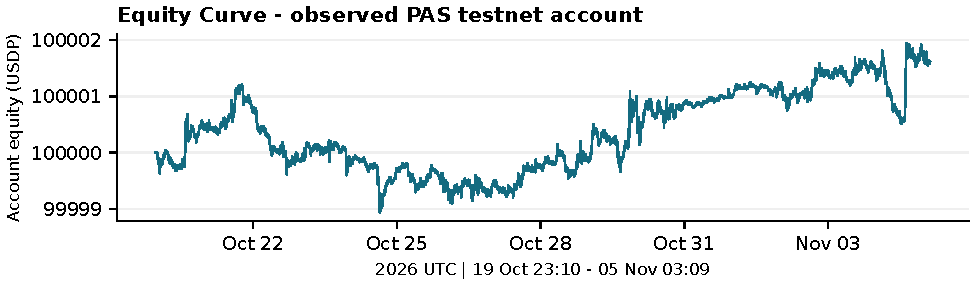
\includegraphics[width=.92\linewidth]{figures/pas-equity-curve.pdf}
\par\small Figure 1. Actual saved account equity; 21,251 observations. No simulated values.
\vspace{2mm}
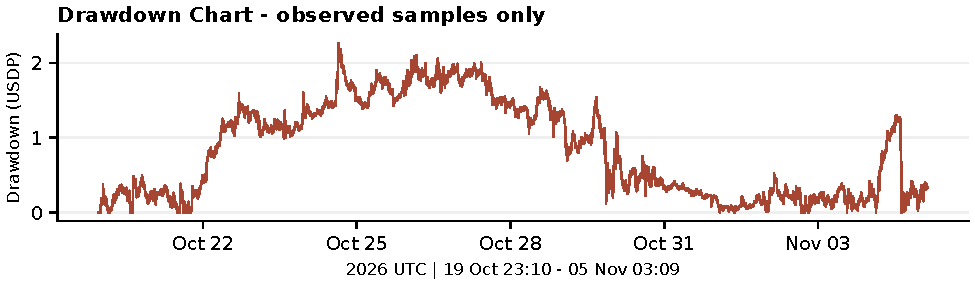
\includegraphics[width=.92\linewidth]{figures/pas-drawdown.pdf}
\par\small Figure 2. $D_t=\max_{u\le t}E_u-E_t$; sampled maximum 2.266909 USDP
\par\small (0.002266882\% of the running peak). Four gaps over five minutes are unconnected.
\end{center}
\newpage

\section{Limitations and future work}
The main contribution is execution reliability and reproducible rejection of weak hypotheses, not established new alpha. Tiny exposure (25/100,000 = 0.025\% of baseline equity) makes account return a poor standalone comparison with teams using larger allocations. ETH directional risk, funding regime changes, API failures and wide spreads can impair the baseline.

The figures cover 19 October 23:10 to 5 November 03:09 UTC, not the full competition. Observations are roughly one minute apart, with four gaps longer than five minutes (longest 22.17 minutes). Recorded drawdown therefore cannot establish the true intraperiod maximum. This earlier snapshot was selected for reporting although later observations existed at report preparation; the positive interim result must not be presented as current or final performance. Final official rank and a complete external intervention/transfer audit remain unavailable. We do not extrapolate the curve. Historical USDP scenario profits are distinct from observed account returns.

Prospective validation, full account attribution and a separately accepted predictive layer remain future work.

\section{Use of AI assistants}
AI assistants, including Codex, helped implement code, tests, research scripts and documentation, and prepare this report. This report's source checks and account arithmetic are documented separately. The dedicated live Funding-LAST runner is deterministic; no LLM selected its orders. General Agent/LLM integration remained experimental.

\section{Open section}
\textbf{Research evolution (overlapping workstreams).} Initial strategy exploration asked whether visible persistence, reversals, funding imbalances or oracle dislocations contained an edge. Basis work changed the question from ``did price move correctly?'' to ``could a position enter and exit after costs?'' Longer-history revalidation then challenged the apparent short-window winners. These results motivated stronger comparisons and support requirements, not the claim that all such signals are universally ineffective [E3, E8].

\textbf{Agent-based selection.} The teammate's candidate-generation/model-selection/risk architecture separated economic rules from allocation and made abstention explicit. Its research question was whether selection added value to existing signals, not whether an unconstrained LLM could invent and sign trades. Separately, PR~20's frozen regime selector stayed flat under its support/validation gates: insufficient evidence, not proof that regimes contain no information. The Agent's small, repeatedly inspected paper sample did not establish incremental value; a validated PAS signing/reconciliation bridge was also absent. It therefore remained offline [E7, E9].

\textbf{Robust infrastructure and reproducible validation.} In parallel, we retained a simple, interpretable Funding-LAST live baseline and concentrated engineering on independent risk admission, durable intents and exchange reconciliation. The common \texttt{ForecastProducer}/\texttt{AgentAdapter}, Core/Worker, scoped Data Gateway and Synthetic Paper framework provided separate test boundaries, not live model authority [E1, E6]. PR~27's new-segment short-cycle scenarios failed after costs; PR~38 formalized frozen hypotheses and retained negative/insufficient outcomes. H09 then tested incremental prediction against a baseline and stopped on failure. These overlapping efforts turned exploration into auditable acceptance gates [E4, E10].

\begin{center}\small
\fbox{Market phenomenon}\ $\longrightarrow$\ \fbox{Fixed signal / baseline}\ $\longrightarrow$\ \fbox{Time / quality checks}\\[2mm]
\hspace*{8mm}$\longrightarrow$\ \fbox{Costs / robustness}\ $\longrightarrow$\ \fbox{Accept / reject / insufficient evidence}
\end{center}
The technical outcome is a risk-controlled execution system and a reproducible research workflow. Complex selection, historical profit and price correlation each required their own evidence; none justified promoting an unvalidated model into the trading wallet.

\appendix
\section{Appendix}
\small
\textbf{Evidence key.} E1--E2: historical runner/deployment; E3: PR~15; E4: PR~43; E5: archived 5 November account snapshot; E6: common framework; E7: PR~31 Agent; E8: basis study; E9: PR~20; E10: PR~27/38. Exact revisions, paths, hashes and limitations: accompanying \texttt{report-evidence-checklist.md}.
\end{document}
